\section{Sprint 2 : Gestion des machines et des équipements}

\subsection{Introduction}

Après la mise en place de l'authentification et du contrôle des accès, ce deuxième Sprint est consacré à la structuration du parc industriel. Il porte sur la gestion des machines, de leurs types, des modules qui les composent, des capteurs associés ainsi que des documents techniques.

Cette étape constitue le socle fonctionnel de la plateforme. Les plans de maintenance préventive, les pannes, les ordres de travail, les interventions et les analyses d'anomalies sont tous rattachés à une machine et, selon le cas, à l'un de ses modules. La qualité de cette structuration conditionne donc la traçabilité des opérations réalisées dans les Sprints suivants.

Ce chapitre présente les objectifs et le Sprint Backlog, puis la conception du domaine des équipements. Il décrit ensuite les fonctionnalités réalisées, notamment la fiche machine, l'historique, la gestion documentaire et le versionnement des documents, avant de présenter les tests de validation.

\subsection{Objectifs du Sprint}

L'objectif principal de ce Sprint est de construire un référentiel fiable des équipements industriels d'IPROTEX Tunisie et de permettre la consultation de leurs informations techniques.

Les objectifs spécifiques sont les suivants :

\begin{itemize}
    \item gérer les machines et leurs types ;
    \item gérer les modules, les types de modules et les composants associés ;
    \item représenter la décomposition hiérarchique d'une machine en modules et sous-modules ;
    \item associer des capteurs aux modules et conserver les mesures collectées ;
    \item consulter la fiche descriptive et l'historique d'une machine ;
    \item téléverser, valider, publier et archiver les documents techniques ;
    \item associer les manuels et documents aux machines concernées ;
    \item gérer les versions successives d'un document ;
    \item contrôler l'accès aux documents selon le rôle de l'utilisateur.
\end{itemize}

À la fin du Sprint, l'administrateur doit pouvoir structurer le parc industriel et la documentation technique, tandis que les techniciens et les opérateurs doivent pouvoir consulter les informations nécessaires à leurs interventions.

\subsection{Sprint Backlog}

Le tableau~\ref{tab:sprint2-backlog} recense les tâches planifiées pour ce Sprint.

{\small
\setlength{\tabcolsep}{5pt}
\begin{longtable}{|p{1cm}|p{10.3cm}|p{1.5cm}|p{1.4cm}|}
\caption{Sprint Backlog du Sprint 2}
\label{tab:sprint2-backlog}\\
\hline
\textbf{ID} & \textbf{Tâche} & \textbf{Priorité} & \textbf{Statut} \\
\hline
\endfirsthead

\hline
\textbf{ID} & \textbf{Tâche} & \textbf{Priorité} & \textbf{Statut} \\
\hline
\endhead

S2-01 &
Développer le référentiel des types de machines. &
Haute & Réalisé \\
\hline

S2-02 &
Développer la gestion des machines et de leurs informations descriptives. &
Haute & Réalisé \\
\hline

S2-03 &
Développer les types de modules et la gestion des modules. &
Haute & Réalisé \\
\hline

S2-04 &
Gérer la hiérarchie des modules et les pièces associées. &
Moyenne & Réalisé \\
\hline

S2-05 &
Associer les capteurs aux modules et conserver les mesures. &
Moyenne & Réalisé \\
\hline

S2-06 &
Développer la fiche machine et la chronologie des événements. &
Haute & Réalisé \\
\hline

S2-07 &
Mettre en place le téléversement et le versionnement des documents. &
Haute & Réalisé \\
\hline

S2-08 &
Gérer la validation, la publication et l'archivage des documents. &
Moyenne & Réalisé \\
\hline

S2-09 &
Développer la consultation sécurisée des manuels et des aperçus. &
Haute & Réalisé \\
\hline

S2-10 &
Vérifier les fonctionnalités par des tests d'API et des tests automatisés. &
Haute & Réalisé \\
\hline

\end{longtable}}

\subsection{User Stories du Sprint}

Les fonctionnalités de ce Sprint sont décrites sous la forme des User Stories suivantes :

{\small
\begin{itemize}
    \item \textbf{US07 :} en tant qu'administrateur, je souhaite gérer les machines et leurs types afin de constituer un référentiel du parc industriel ;
    \item \textbf{US08 :} en tant qu'administrateur, je souhaite gérer les modules et leurs types afin de décrire la structure des équipements ;
    \item \textbf{US09 :} en tant qu'utilisateur autorisé, je souhaite consulter la fiche et l'historique d'une machine afin de préparer une intervention ;
    \item \textbf{US10 :} en tant qu'administrateur, je souhaite téléverser et versionner les documents techniques afin de disposer d'une documentation à jour ;
    \item \textbf{US11 :} en tant que technicien ou opérateur, je souhaite consulter les manuels publiés afin de m'appuyer sur les procédures constructeur.
\end{itemize}}

\subsection{Conception du Sprint}

\subsubsection{Diagramme des cas d'utilisation}

Le diagramme de la figure~\ref{fig:usecase-machines} présente les cas d'utilisation associés à la gestion des équipements. L'administrateur dispose des fonctions de création et de structuration du référentiel : types de machines, machines, modules, capteurs et documents techniques. Les techniciens et les opérateurs accèdent à la fiche machine, à l'historique ainsi qu'aux manuels publiés, sans pouvoir modifier le référentiel.

\begin{figure}[H]
    \centering
    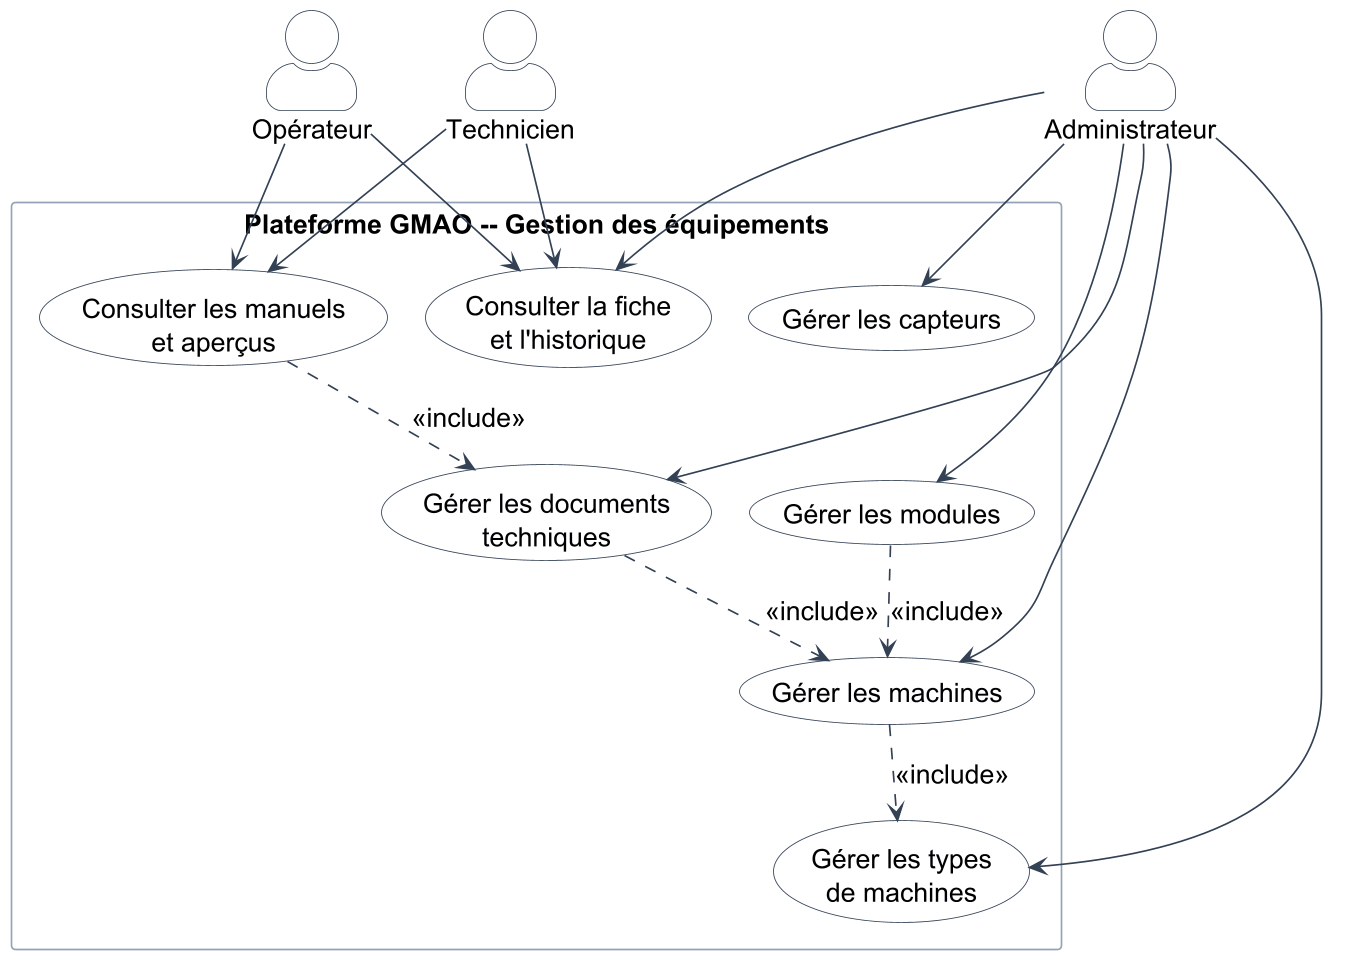
\includegraphics[width=0.80\textwidth,height=0.45\textheight,keepaspectratio]{figures/usecase-machines.png}
    \caption{Diagramme des cas d'utilisation du Sprint 2}
    \label{fig:usecase-machines}
\end{figure}

Les relations d'inclusion traduisent les dépendances du domaine : la gestion d'une machine suppose l'existence de son type, la gestion des modules s'appuie sur les machines, l'association des documents se fait au niveau d'une machine et la consultation des manuels passe par les documents publiés.

\subsubsection{Diagramme de classes du domaine}

La figure~\ref{fig:classes-machines} présente les entités du domaine des équipements.

\begin{figure}[H]
    \centering
    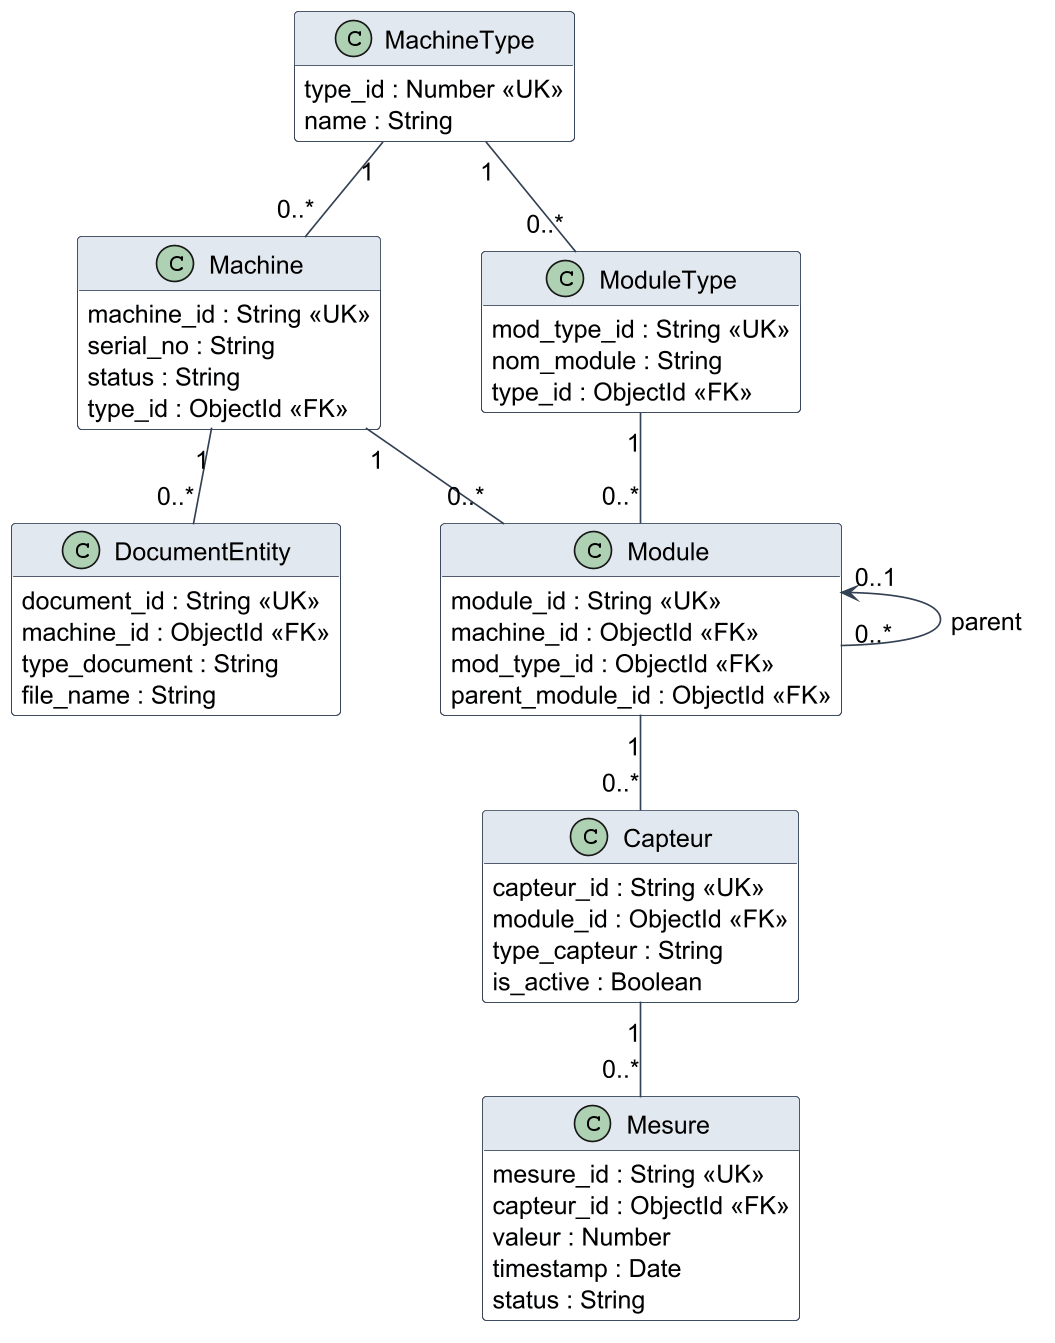
\includegraphics[
        width=\textwidth,
        height=0.57\textheight,
        keepaspectratio
    ]{figures/classes-machines.png}
    \caption{Diagramme de classes du domaine des équipements}
    \label{fig:classes-machines}
\end{figure}

Une machine appartient à un type donné et peut contenir plusieurs modules. Ces modules sont décrits par un type et peuvent être organisés de manière hiérarchique au moyen d'un module parent. Chaque module peut être associé à des capteurs, lesquels produisent des mesures horodatées. Les documents techniques sont rattachés à la machine concernée.

Les identifiants marqués \texttt{<UK>} correspondent aux clés fonctionnelles des entités, tandis que les attributs marqués \texttt{<FK>} portent les références entre documents MongoDB. La relation réflexive sur \texttt{Module} permet de représenter les sous-modules d'une même machine, ce qui autorise une décomposition progressive des équipements selon leur complexité.

\subsubsection{Diagramme de séquence de la création d'une machine}

L'enregistrement d'une machine est réservé à l'administrateur. La figure~\ref{fig:sequence-machine} présente le contrôle des autorisations, la validation des données et l'enregistrement du document dans la base.

\begin{figure}[H]
    \centering
    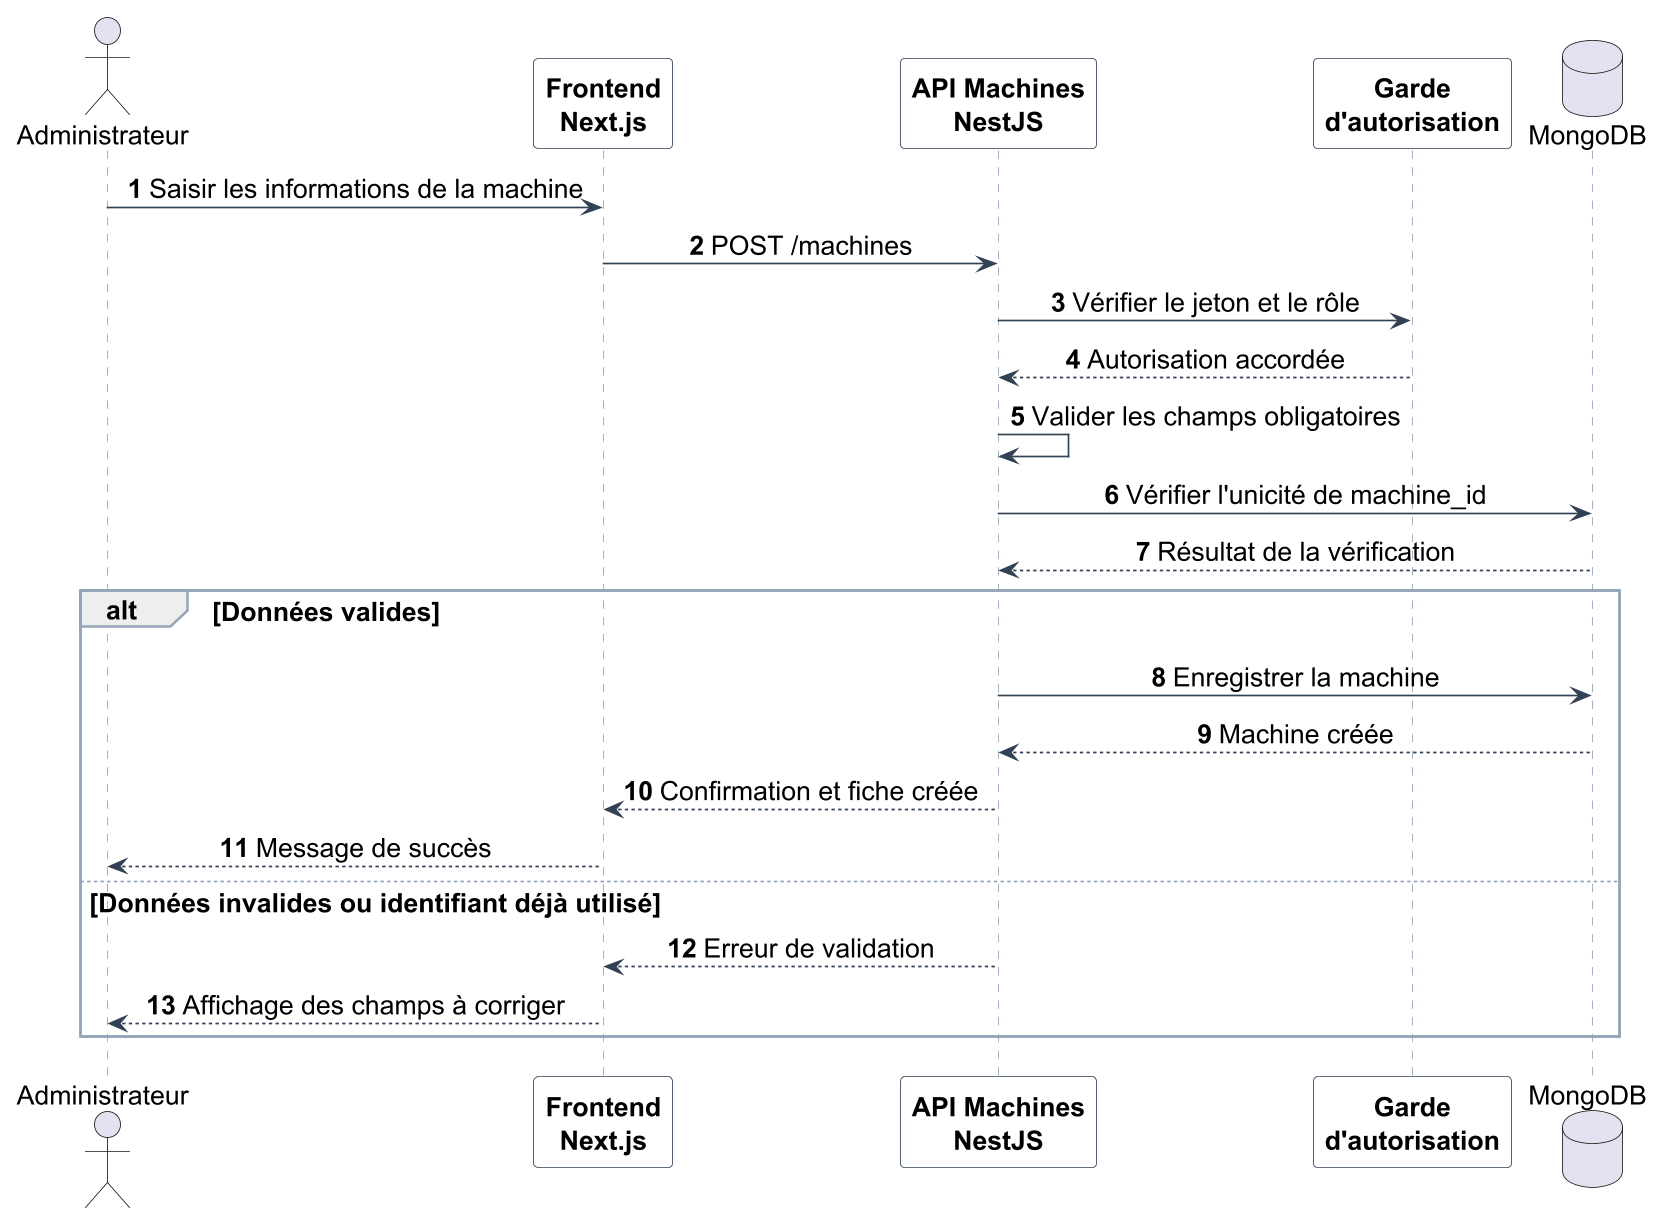
\includegraphics[width=\textwidth,height=0.68\textheight,keepaspectratio]{figures/sequence-create-machine.png}
    \caption{Diagramme de séquence de la création d'une machine}
    \label{fig:sequence-machine}
\end{figure}

La requête est d'abord interceptée par le garde d'autorisation, qui vérifie la validité du jeton et le rôle de l'appelant avant d'atteindre le service métier. L'API contrôle ensuite les champs obligatoires et interroge la base pour s'assurer que l'identifiant n'est pas déjà utilisé. Si les données sont valides, la machine est enregistrée et le frontend affiche sa fiche ; sinon, les champs à corriger sont signalés à l'administrateur.

\subsubsection{Modèle de données des équipements}

Le tableau~\ref{tab:modele-equipements} présente les principales entités du domaine et leur rôle.

\begin{table}[H]
\centering
\caption{Entités du domaine des équipements}
\label{tab:modele-equipements}
\small
\begin{tabularx}{\textwidth}{|p{3.1cm}|X|}
\hline
\textbf{Entité} & \textbf{Rôle dans le domaine} \\
\hline
\texttt{MachineType} & Catégorie technique de la machine et référentiel de classification \\
\hline
\texttt{Machine} & Équipement industriel identifié par un identifiant unique et un numéro de série \\
\hline
\texttt{ModuleType} & Type de module rattaché à une catégorie de machine \\
\hline
\texttt{Module} & Composant d'une machine, éventuellement rattaché à un module parent \\
\hline
\texttt{Capteur} & Dispositif de mesure associé à un module \\
\hline
\texttt{Mesure} & Valeur horodatée transmise par un capteur \\
\hline
\texttt{DocumentEntity} & Document technique associé à une machine et soumis à un versionnement \\
\hline
\end{tabularx}
\end{table}

La liste des machines de l'entreprise fournit par ailleurs les informations descriptives du parc : constructeur, année de fabrication et référence produit. Ces données sont intégrées lors de la création ou de l'importation des équipements.

MongoDB étant une base orientée documents, les associations sont matérialisées par des identifiants de référence. Ce choix facilite l'évolution du modèle et reste cohérent avec la structure conceptuelle décrite par le diagramme de classes~\cite{omg_uml,mongodb_atlas_docs}. La couche d'accès aux données s'appuie sur Mongoose, qui fournit les modèles et les références entre documents~\cite{mongoose_docs}.

\subsection{Réalisation}

\subsubsection{Gestion des machines}

Le module des machines permet à l'administrateur de créer, consulter, modifier et supprimer un équipement. Chaque machine est identifiée par un identifiant unique, un numéro de série, un type et un état d'exploitation.

Le formulaire de création regroupe les informations administratives et techniques de l'équipement. Les champs obligatoires sont contrôlés côté client puis validés par l'API. L'unicité de l'identifiant et du numéro de série est vérifiée avant l'enregistrement afin d'éviter les doublons.

La liste des machines propose une recherche, un filtrage par type et par état ainsi qu'une pagination. L'administrateur peut accéder directement à la fiche détaillée de chaque équipement.

% Capture d'écran : déposer le fichier figures/sprint2-machines-list.png pour l'afficher.
\IfFileExists{figures/sprint2-machines-list.png}{%
\begin{figure}[H]
    \centering
    \includegraphics[width=0.95\textwidth,keepaspectratio]{figures/sprint2-machines-list.png}
    \caption{Liste des machines industrielles}
    \label{fig:sprint2-machines-list}
\end{figure}
}{}

\subsubsection{Gestion des modules et des composants}

Une machine peut être décomposée en plusieurs modules, eux-mêmes décrits par un type de module. Cette organisation permet de représenter la structure réelle des équipements, par exemple les ensembles fonctionnels d'une tresseuse ou d'une machine de découpe.

Le modèle prend en charge une hiérarchie de modules au moyen d'un module parent facultatif. Cette possibilité permet de décrire des sous-ensembles lorsque la structure de la machine le nécessite.

L'administrateur peut associer des pièces aux modules afin de préparer le lien avec le catalogue de pièces de rechange utilisé dans le Sprint consacré aux stocks.

Des capteurs peuvent également être rattachés aux modules. Chaque capteur est identifié, typé et activé ou désactivé selon son état de fonctionnement. Les mesures transmises sont horodatées et conservées avec leur statut afin d'être exploitées par le module de surveillance.

\subsubsection{Fiche machine et historique}

La fiche machine regroupe les informations descriptives de l'équipement, ses modules, ses documents techniques et les principaux événements qui le concernent.

La chronologie de la machine rassemble les événements liés aux interventions, aux ordres de travail, aux mesures et aux analyses d'anomalies. Cette vue permet aux techniciens de reconstituer le contexte d'une défaillance et de consulter les actions déjà réalisées sur l'équipement.

L'accès à cette chronologie est limité par le contrôle des autorisations : l'administrateur dispose d'une vue complète, tandis que le technicien et l'opérateur consultent les informations relatives aux machines qui leur sont accessibles.

% Capture d'écran : déposer le fichier figures/sprint2-machine-detail.png pour l'afficher.
\IfFileExists{figures/sprint2-machine-detail.png}{%
\begin{figure}[H]
    \centering
    \includegraphics[width=0.95\textwidth,keepaspectratio]{figures/sprint2-machine-detail.png}
    \caption{Fiche détaillée et chronologie d'une machine}
    \label{fig:sprint2-machine-detail}
\end{figure}
}{}

\subsubsection{Gestion documentaire}

La plateforme permet d'associer des manuels, des notices et d'autres documents techniques aux machines. Chaque document est décrit par un nom, un type et la machine concernée.

Le processus de gestion documentaire comprend le téléversement du fichier, sa validation, sa publication puis, le cas échéant, son archivage. Un document peut faire l'objet de plusieurs versions successives. L'historique des versions permet de revenir sur les modifications et de vérifier le document effectivement publié.

Les fichiers sont conservés dans un espace de stockage dédié~\cite{supabase_storage}. L'accès est contrôlé par le backend, qui vérifie les autorisations avant de délivrer une URL temporaire. Les informations d'authentification du service de stockage ne sont jamais exposées au navigateur.

Afin de préserver la lisibilité du rapport, seuls les principes du versionnement sont présentés ici. Les captures complètes de gestion documentaire peuvent être placées en annexe.

\subsubsection{Consultation des documents}

Les techniciens et les opérateurs peuvent consulter les documents publiés et les manuels associés aux machines. La consultation s'effectue depuis la fiche machine ou depuis un espace documentaire dédié.

Les documents PDF peuvent être affichés directement dans l'interface au moyen d'un visualiseur intégré. Les autres formats sont proposés au téléchargement après vérification des autorisations.

Ce mécanisme évite la diffusion de documents non validés ou archivés et garantit que les utilisateurs disposent de la version en vigueur lors de leurs interventions.

% Capture d'écran : déposer le fichier figures/sprint2-document-viewer.png pour l'afficher.
\IfFileExists{figures/sprint2-document-viewer.png}{%
\begin{figure}[H]
    \centering
    \includegraphics[width=0.9\textwidth,keepaspectratio]{figures/sprint2-document-viewer.png}
    \caption{Consultation d'un document technique dans la plateforme}
    \label{fig:sprint2-document-viewer}
\end{figure}
}{}

\subsection{Tests et validation}

Le tableau~\ref{tab:tests-sprint2} présente une synthèse des scénarios vérifiés pour ce Sprint.

{\footnotesize
\setlength{\tabcolsep}{4pt}
\begin{longtable}{|p{0.9cm}|p{8.6cm}|p{5.6cm}|}
\caption{Scénarios de test du Sprint 2}
\label{tab:tests-sprint2}\\
\hline
\textbf{ID} & \textbf{Scénario} & \textbf{Résultat attendu} \\
\hline
\endfirsthead

\hline
\textbf{ID} & \textbf{Scénario} & \textbf{Résultat attendu} \\
\hline
\endhead

T2-01 &
Création d'une machine avec des données valides &
Machine enregistrée et visible dans la liste \\
\hline

T2-02 &
Création d'une machine avec un identifiant déjà utilisé &
Enregistrement refusé avec message explicite \\
\hline

T2-03 &
Création d'une machine sans champ obligatoire &
Validation refusée et champs signalés \\
\hline

T2-04 &
Création d'un module rattaché à une machine &
Module enregistré et affiché dans la fiche machine \\
\hline

T2-05 &
Création d'un sous-module &
Hiérarchie conservée et affichée correctement \\
\hline

T2-06 &
Association d'un capteur à un module &
Capteur visible et disponible pour la collecte \\
\hline

T2-07 &
Consultation de la fiche machine par un technicien &
Informations autorisées affichées \\
\hline

T2-08 &
Téléversement d'un document technique &
Document enregistré et associé à la machine \\
\hline

T2-09 &
Publication d'une nouvelle version d'un document &
Version publiée et ancienne version conservée \\
\hline

T2-10 &
Consultation d'un document archivé &
Accès refusé \\
\hline

T2-11 &
Tentative de gestion des machines par un opérateur &
Requête refusée par le contrôle des autorisations \\
\hline

\end{longtable}}

Les tests d'API ont confirmé la validation des données, le contrôle des autorisations et l'unicité des identifiants. Les tests automatisés du frontend couvrent notamment la logique de la fiche machine, du visualiseur de documents et de la gestion des manuels. Les anomalies détectées ont été corrigées avant la revue du Sprint.

\subsection{Revue du Sprint et conclusion}

Lors de la revue, le référentiel des machines, la gestion des modules, la fiche machine, la chronologie et le processus documentaire ont été présentés. Le contrôle des accès aux documents a également été vérifié pour les trois profils.

Les principaux résultats du Sprint sont les suivants :

\begin{itemize}
    \item constitution d'un référentiel structuré des machines et de leurs types ;
    \item décomposition des équipements en modules et sous-modules ;
    \item association des capteurs et conservation des mesures ;
    \item consultation centralisée de la fiche et de l'historique d'une machine ;
    \item gestion documentaire avec validation, publication, archivage et versionnement ;
    \item consultation sécurisée des manuels et des documents techniques.
\end{itemize}

La rétrospective a souligné l'importance de cette étape : la majorité des fonctionnalités suivantes s'appuient sur les machines et les modules créés dans ce Sprint.

Le Sprint 3 sera consacré à la gestion de la maintenance préventive, depuis les plans et les listes de contrôle jusqu'à la validation des interventions et à la génération automatique de la prochaine échéance.
